\documentclass[11pt,a4paper]{article}
\usepackage[utf8]{inputenc}
\usepackage[spanish]{babel}	%Idioma
\usepackage{amsmath}
\usepackage{amsfonts}
\usepackage{amssymb}
\usepackage{graphicx} 	%Añadir imágenes
\usepackage{geometry}	%Ajustar márgenes
\usepackage[export]{adjustbox}[2011/08/13]
\usepackage{float}
\restylefloat{table}
\usepackage[hidelinks]{hyperref}
\usepackage{titling}
\usepackage{multirow}
\usepackage{caption}
\usepackage{multicol}
\usepackage[shortlabels]{enumitem}
\usepackage{array}
\selectlanguage{spanish}

%Opciones de encabezado y pie de página:
\usepackage{fancyhdr}
\pagestyle{fancy}
\lhead{Nazaret Román Guerrero}
\rhead{Sistemas Gráficos}
\lfoot{Grado en Ingeniería Informática}
\cfoot{}
\rfoot{\thepage}
\renewcommand{\headrulewidth}{0.4pt}
\renewcommand{\footrulewidth}{0.4pt}

%Opciones de fuente:
\usepackage[utf8]{inputenc}
\usepackage[default]{sourcesanspro}
\usepackage{sourcecodepro}
\usepackage[T1]{fontenc}

\setlength{\parindent}{15pt}
\setlength{\headheight}{15pt}
\setlength{\voffset}{10mm}

% Custom colors
\usepackage{color}
\definecolor{deepblue}{rgb}{0,0,0.5}
\definecolor{deepred}{rgb}{0.6,0,0}
\definecolor{deepgreen}{rgb}{0,0.5,0}
\definecolor{morado}{rgb}{0.4,0,0.8}

\usepackage{listings}

\begin{document}
\begin{titlepage}

\begin{minipage}{\textwidth}

\centering

\includegraphics[width=0.5\textwidth]{img/logo.png}\\

\textsc{\Large Sistemas Gráficos\\[0.2cm]}
\textsc{GRADO EN INGENIERÍA INFORMÁTICA}\\[1cm]

{\Huge\bfseries Diseño de la aplicación\\}
\noindent\rule[-1ex]{\textwidth}{3pt}\\[3.5ex]
{\large\bfseries Bleach RPG}
\end{minipage}

\vspace{1.5cm}
\begin{minipage}{\textwidth}
\centering

\textbf{Autora}\\ {Nazaret Román Guerrero}\\[2.5ex]

\includegraphics[width=0.3\textwidth]{img/etsiit.jpeg}\\[0.1cm]
\vspace{1cm}
\textsc{Escuela Técnica Superior de Ingenierías Informática y de Telecomunicación}\\
\vspace{1cm}
\textsc{Curso 2019-2020}
\end{minipage}
\end{titlepage}

\pagenumbering{gobble}
\pagenumbering{arabic}
\tableofcontents
\thispagestyle{empty}

\newpage

\section{Consideraciones iniciales}

Este juego está basado en una serie, \textit{Bleach}, donde el personaje principal, Kurosaki Ichigo debe luchar contra varios personajes para salvar a sus amigos y a sí mismo. En el transcurso de la serie debe recuperar el alma de una de sus amigas y para ello debe luchar contra Grimmjow  Jaegerjaquez, un \textit{Adjuchas} (pronunciado como Adyukas) que es muy peligroso y poderoso.\\

Para adaptar esto al juego, he cambiado ligeramente el alma y he obligado a que Ichigo deba recuperar su propia alma, de forma que el combate no sea equilibrado sino que tenga cierta desventaja para nuestro personaje.

\section{Análisis de requisitos}

Para explicar lo que debe hacer la aplicación se han definido unos requisitos funcionales que son los siguientes:

\begin{itemize}
	\item RF1. Habrá un personaje principal para controlar y un enemigo contra el que luchar.
	\item RF2. El protagonista podrá moverse por el escenario.
	\item RF3. Los movimientos estarán restringidos a la zona de suelo del escenario.
	\item RF4. El protagonista podrá atacar al enemigo.
	\item RF5. Cada personaje tendrá puntos de vida.
	\item RF6. Los puntos de vida de cada uno se verán en la pantalla en todo momento.
	\item RF7. Se indicará cuando el personaje ha ganado o perdido.
\end{itemize}

\subsection{Explicación de cada requisito}

\begin{itemize}
	\item RF1. El personaje principal será Ichigo, cuyo objetivo será recuperar un objeto.
	\item RF2. El personaje podrá moverse mediante el uso de las teclas \color{morado}\texttt{asdw}\color{black}.
	\item RF3. Ninguno de los personajes podrá salirse del área de combate; este área estará restringida por paredes físicas que impedirán el paso más allá.
	\item RF4. Para poder conseguir el objeto, el personaje podrá atacar al enemigo mediante clicks de ratón.
	\item RF5. Cada personaje tendrá una vida limitada y cuando ésta llegue a 0, el personaje habrá muerto.
	\item RF6. Habrá un display con la vida de cada personaje que se actualizará cada vez que un personaje ataque al otro.
	\item RF7. Cuando el personaje principal gane o pierda, se alertará desde el navegador con el resultado de la batalla.
\end{itemize}

\section{Codificación}

Para llevar a cabo la funcionalidad requerida se ha creado un diagrama de clases para explicar cómo está implementada la aplicación a partir de él.

\begin{figure}[H]
	\centering
	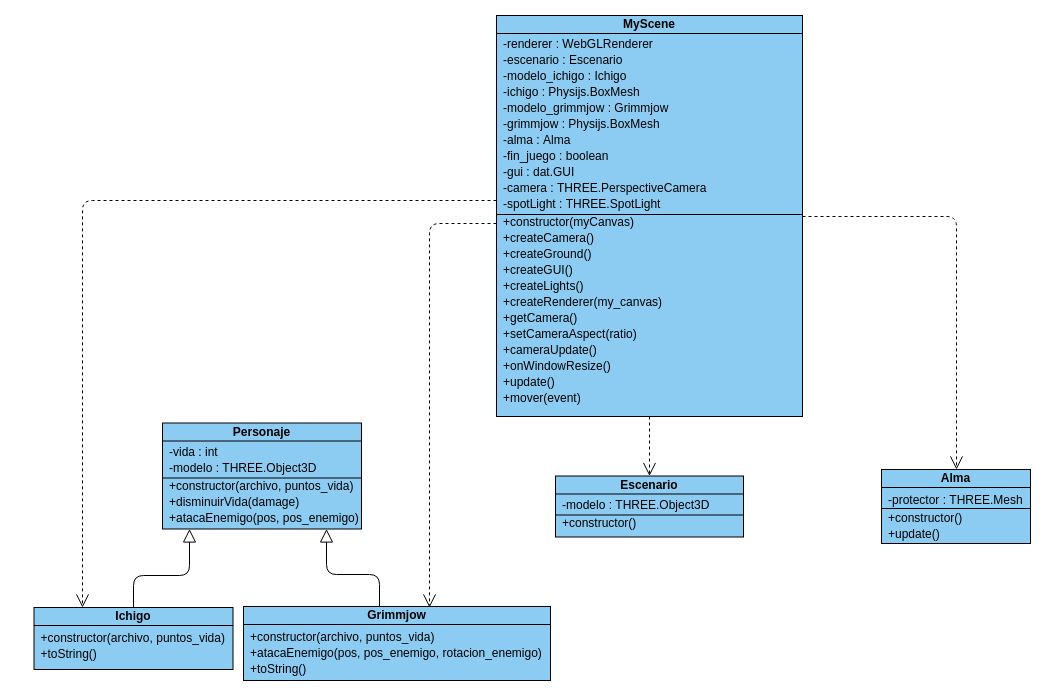
\includegraphics[scale=0.4]{img/diagrama.png}
\end{figure}

Como podemos ver, hay una clase principal, \texttt{MyScene}, que se encarga de unir y renderizar los personajes, el escenario y el objeto (el alma) que se debe recuperar para completar el juego.\\

Los personajes \texttt{Ichigo} y \texttt{Grimmjow} descienden de una clase padre \texttt{Personaje}, donde está el atributo de la vida del personaje y los métodos para cargar el archivo del modelo y los materiales, para gestionar la disminución de vida (y la muerte) cuando el enemigo hace daño y el método para golpear al enemigo.\\

Los modelos de los personajes han sido sacados de los siguientes enlaces:

\begin{itemize}
	\item \textbf{Ichigo}: \color{blue}\url{https://www.models-resource.com/wii/bleachversuscrusade/model/44/}\color{black}.
	\item \textbf{Grimmjow}: \color{blue}\url{https://www.models-resource.com/wii/bleachversuscrusade/model/48/}\color{black}.
\end{itemize}

\section{Simulación con físicas}

Para poder gestionar algunos de los requisitos, como el ataque o la restricción de los personajes al área de lucha se ha utilizado el motor de físicas de las transparencias de clase, el motor \texttt{Physijs}.\\

Los personajes han sido rodeados con una caja física para simular que son objetos físicos y no simples modelos. 
Además, se ha creado una estructura que une un suelo con cuatro paredes para que no caminen más allá del escenario. Esto puede observarse en la siguiente imagen, donde tanto las paredes, el suelo como las cajas de los personajes no se han dejado totalmente transparentes para que se pudiera ver:

\begin{figure}[H]
	\centering
	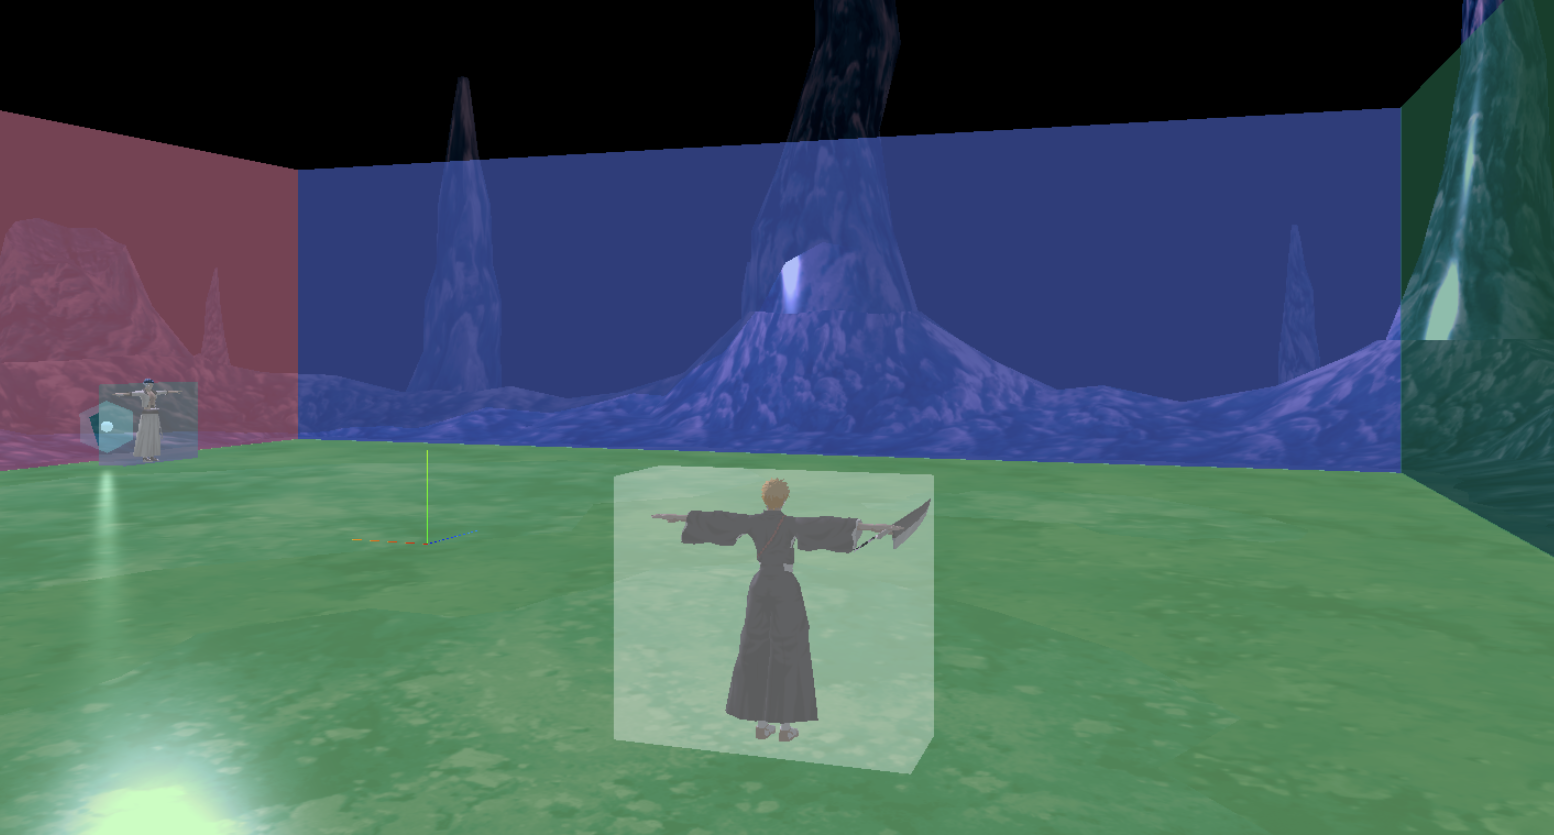
\includegraphics[scale=0.27]{img/fisica.png}
\end{figure}

Por otro lado, el objeto que se ha de recuperar (el alma de nuestro personaje), es una malla de THREEjs simple, no es un objeto físico puesto que no es necesario que lo sea.\\

Dejando el escenario con todas las cajas transparentes, la apariencia de la aplicació es esta:

\begin{figure}[H]
	\centering
	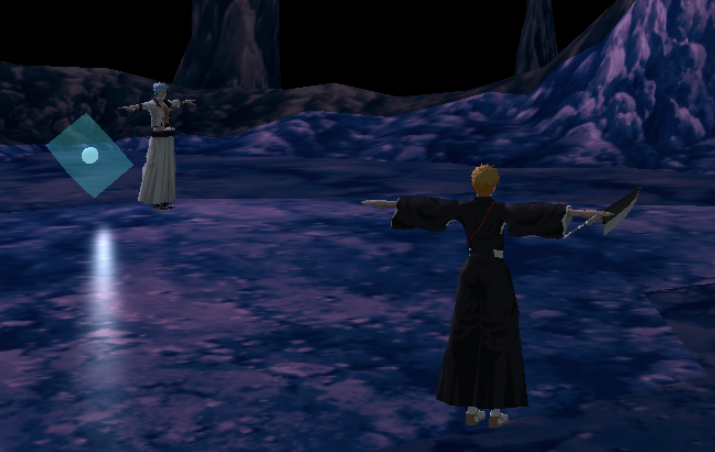
\includegraphics[scale=0.37]{img/inicio.png}
\end{figure}

Los ataques de los personajes se llevan a cabo cuando ambos están en un rango de 5 unidades y se gestionan mediante colisiones. Cuando los personajes chocan se hacen daño mutuamente, un daño aleatorio entre 1 y 3 (ambos incluidos). Por tanto, cuando el personaje principal ataca, también recibirá un daño de vuelta.

\section{Control de la vida}

Para poder ver la vida del personaje se ha utilizado la propia interfaz de usuario. En cada frame se actualizan las barras de vida de cada personaje si se ha producido un ataque y se ha reducido la vida. El aspecto es el siguiente:

\begin{figure}[H]
	\centering
	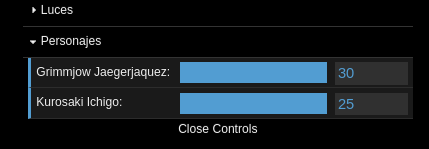
\includegraphics[scale=0.5]{img/barravida.png}
\end{figure}

El enemigo, Grimmjow, tiene un handicap ya que tiene 5 puntos de vida más que el protagonista. Esto está hecho para añadir una cierta dificultad en ganarle y como parte de la historia, ya que el alma del protagonista ha sido robada y eso le ha quitado fuerza vital (he intentado resemblar lo que ocurren en la serie en la que me he basado para hacer este juego).

\end{document}